\documentclass{beamer}
\usetheme{Madrid}
\usepackage{amsmath}
\usepackage{graphicx}
\usepackage{booktabs}
\usepackage{hyperref}

\title{Does Monetary Policy Matter?}
\subtitle{A Narrative Approach to Monetary Policy }
\author{Liming Lin}
\institute{Sciences Po}
\date{\today}

% Show mini TOC at start of each section
\AtBeginSection[]{
  \begin{frame}{Outline}
    \tableofcontents[currentsection]
  \end{frame}
}

\begin{document}

% Title Slide
\begin{frame}
  \titlepage
\end{frame}

% Define all sections BEFORE the TOC frame so it's populated

% Full TOC now works
\begin{frame}{Outline}
  \tableofcontents
\end{frame}

% ========== SECTION: Motivation ==========
\section{Motivation for the Narrative Approach}

\begin{frame}{Why Identification is Hard}
  \begin{itemize}
    \item Goal: Evaluate causal effects of monetary policy
    \[
  Y_t = \alpha + \beta MP_t + \epsilon_t
  \]
    \item Problem: Endogeneity and omitted variables
    \item Example 1: $MP_t$ is a function of $Y_t$
    \[
    MP_t = \gamma + \delta Y_t + \eta_t
    \]
    \item Example 2: $Y_t$ is a function of $MP_t$ and some other variables
    \[
    Y_t = \alpha + \beta MP_t + \gamma X_t + \epsilon_t
    \]
  \end{itemize}
  
  \textit{In either cases, we cannot identify the causal effect of monetary policy on the economy.}
\end{frame}

% ========== SECTION: Narrative Approach ==========
\section{Narrative Approach}

\begin{frame}{What is the Narrative Approach?}
  \begin{itemize}
    \item Identify exogenous shocks from text records
    \begin{itemize}
    \item Use The Federal Open Market Committee (FOMC) transcripts of its meetings on deciding monetary policy
    \item The full transcripts released with 5 years lag, encouraging participants to speak freely
    \item The transcripts are compiled by the officials at the Fed and thus reliable
    \end{itemize}

  \end{itemize}
\end{frame}

\begin{frame}{Criteria for Exogenous Shocks}
    A shock is identified as exogenous if both of the following arguments are mentioned in the transcripts:
  \begin{enumerate}
    \item ``Current Level of Inflation/Unemployment is Unacceptable"
    \item ``Be willing to Accept a Recession/Higher Inflation as consequences of the policy changes" 
  \end{enumerate}
  In other words, its a preference shock that is not driven by the current state of the economy.
\end{frame}

% ========== SECTION: Examples of Shocks ==========
\section{Examples of Shocks}

\begin{frame}{December 1988 (Contractionary)}
  \begin{itemize}
    \item Fed focused on inflation control and was willing to accept recession risk
    \item “In terms of our own inflation rate ... we have been stalled at a rate that I think is too high  for most of us” (W. Lee Hoskins, Transcript, May 17, 1988, p. 5).
    \item However, the inflation and GDP growth rates did not experience a significant change at that time.
  \end{itemize}

\end{frame}
\begin{frame}{December 1988 (Contractionary)}
  \centering
  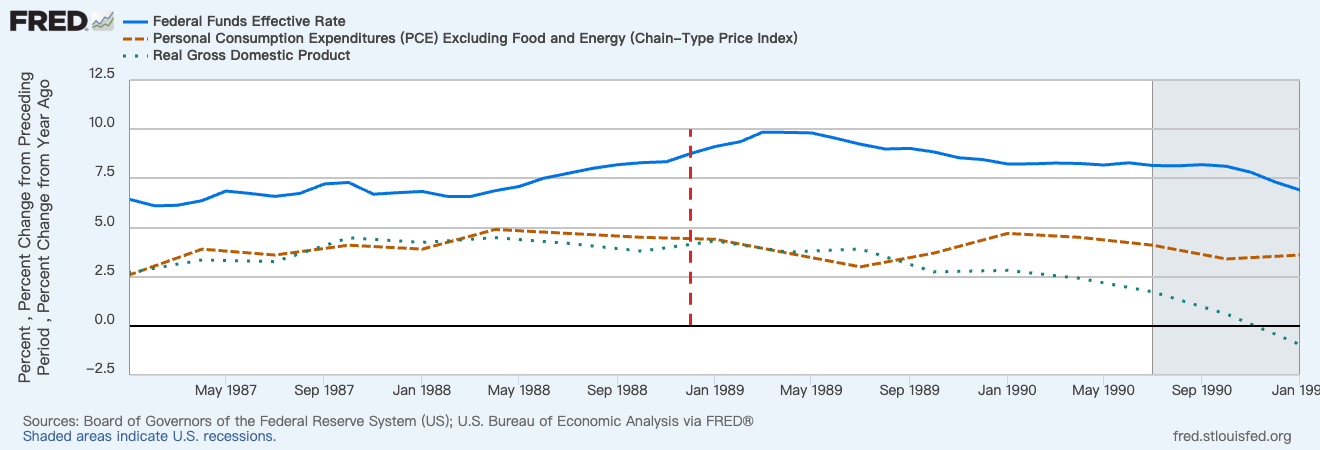
\includegraphics[width=1\linewidth]{Graphs/Dec1988Shocks.png}
\end{frame}

\begin{frame}{January 1972 (Expansionary)}
  \begin{itemize}
    \item Fed focused on high unemployment and was willing to accept higher inflation
    \item “believed the appropriate posture for the System at this point was one of doing what it could with the policy instruments at its disposal to foster and encourage  economic expansion” (J. Dewey Daane, Memorandum of Discussion, December 14, 1971, p. 60).
    \item Again, the unemployment rate has not changed significantly at that time and the inflation even decreased in the previous months.
  \end{itemize}

\end{frame}
\begin{frame}{January 1972 (Expansionary)}
  \centering
  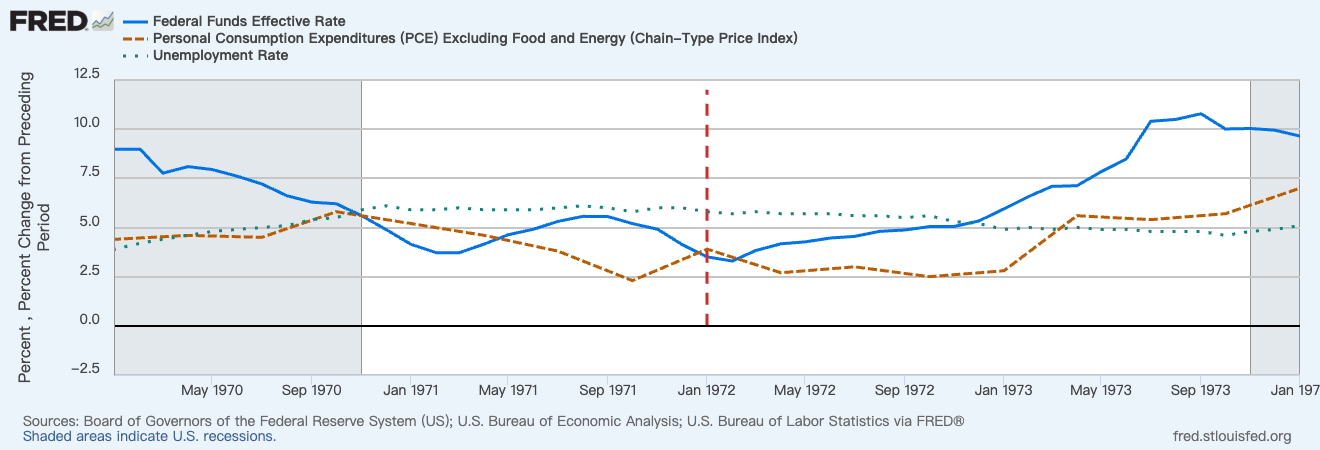
\includegraphics[width=1\linewidth]{Graphs/Jan1972Shocks.png}
\end{frame}
\begin{frame}{Summary of Shocks}
  \begin{itemize}
    \item Nine contractionary, one expansionary shock (1946–2016)
    \item Identified via consistent narrative standards
  \end{itemize}
  \centering
  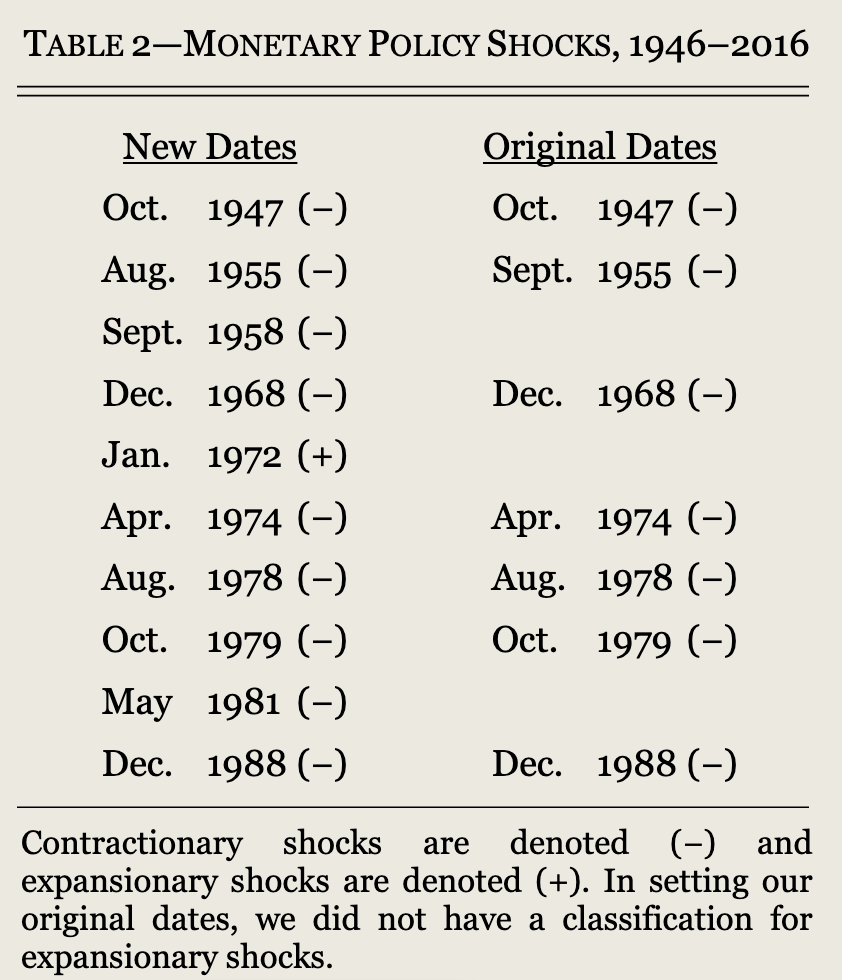
\includegraphics[height=0.6\textheight]{Graphs/Summary of Identified Shocks.png}
\end{frame}

% ========== SECTION: Modeling and Results ==========
\section{Modeling and Results}

\begin{frame}{Jordà’s Local Projection Method}
    \textbf{Purpose:} Estimate impulse responses of variables (e.g., GDP, inflation) to a monetary policy shock, without relying on a full system of equations.
  
    \vspace{1em}
    \textbf{Equation:}
    \[
      Y_{t+h} = \alpha_h + \beta_h \cdot Shock_t + \sum_{k=1}^{p} \phi_{k,h} \cdot Y_{t-k} + \sum_{k=0}^{q} \gamma_{k,h} \cdot Shock_{t-k} + \varepsilon_{t+h}
    \]

    \textbf{Components:}
    \begin{itemize}
      \item $Y_{t+h}$: GDP with $h$ periods ahead
      \item $Shock_t$: Narrative monetary policy shock at time $t$
      \item $\beta_h$: Estimated effect of the shock on $Y$ after $h$ periods (the impulse response)
      \item Lag terms: Control for past outcomes and shocks
    \end{itemize}
  
    \vspace{0.5em}
    \textbf{Key Feature:} One regression per horizon $h$ — no need to invert a VAR.
  
  \end{frame}

\begin{frame}{Response of Unemployment}
  \begin{itemize}
    \item Unemployment ↑ by 1.6 pp after 27 months
  \end{itemize}
  \centering
  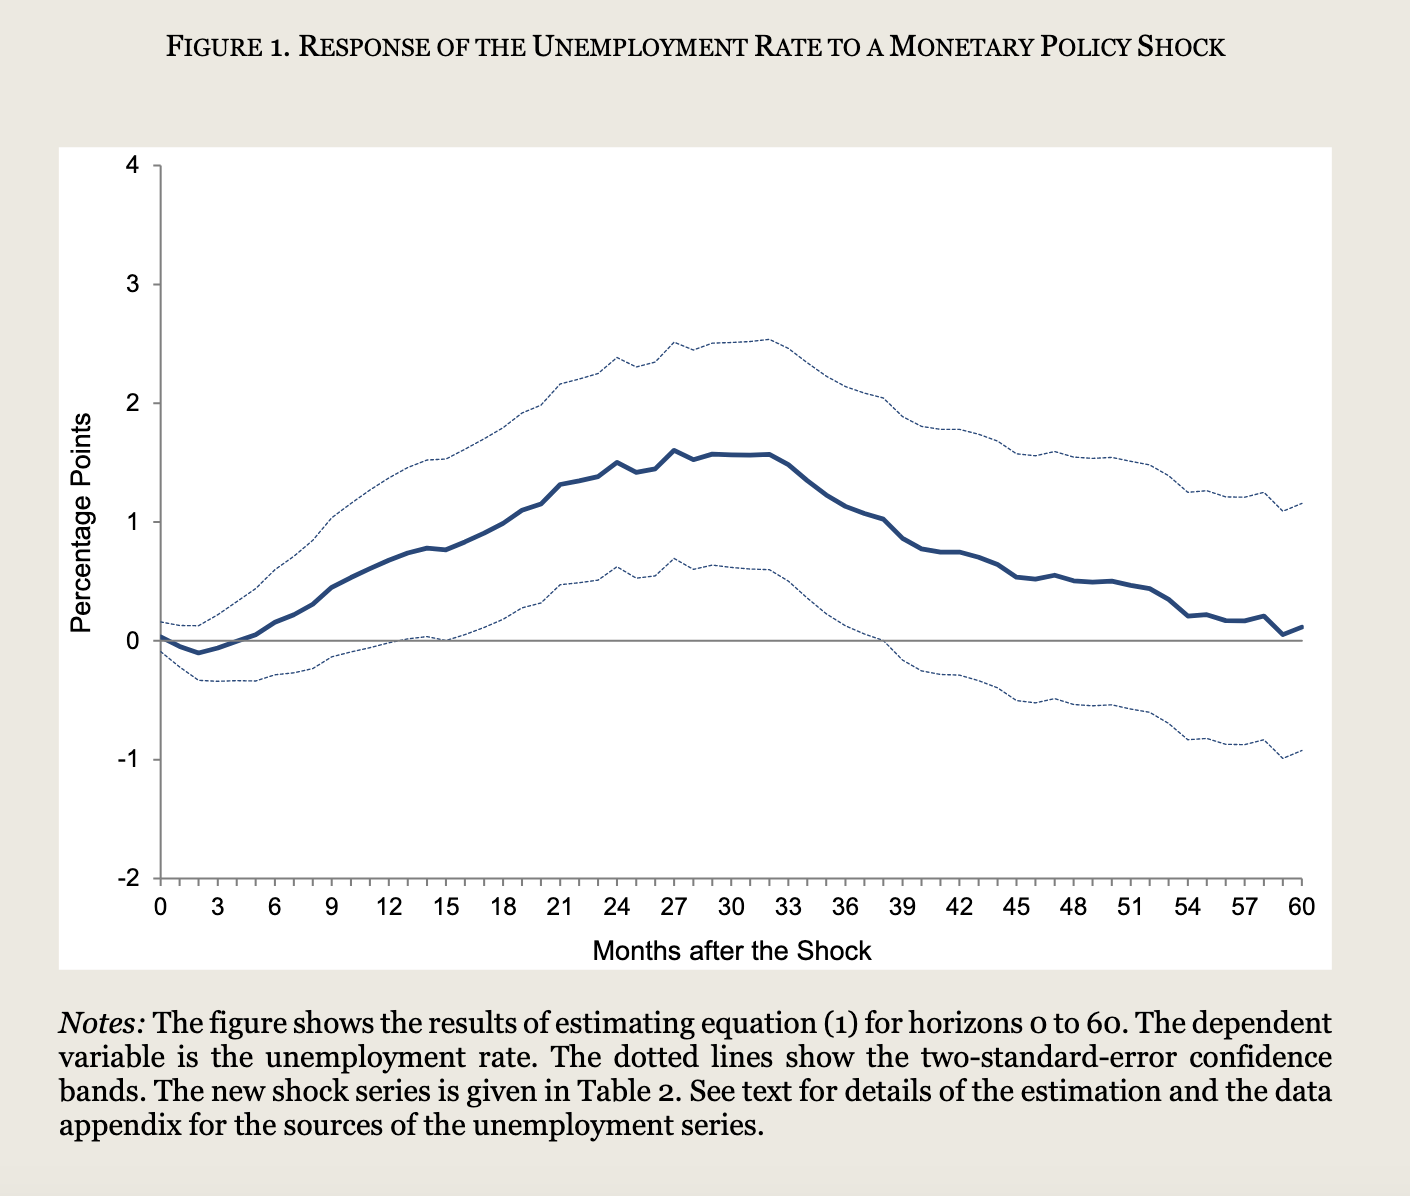
\includegraphics[height=1\textheight]{Graphs/Unemployment Response.png}
\end{frame}

\begin{frame}{Response of Inflation}
  \begin{itemize}
    \item Inflation ↓ by 1.5 pp after 9 quarters
  \end{itemize}
  \centering
  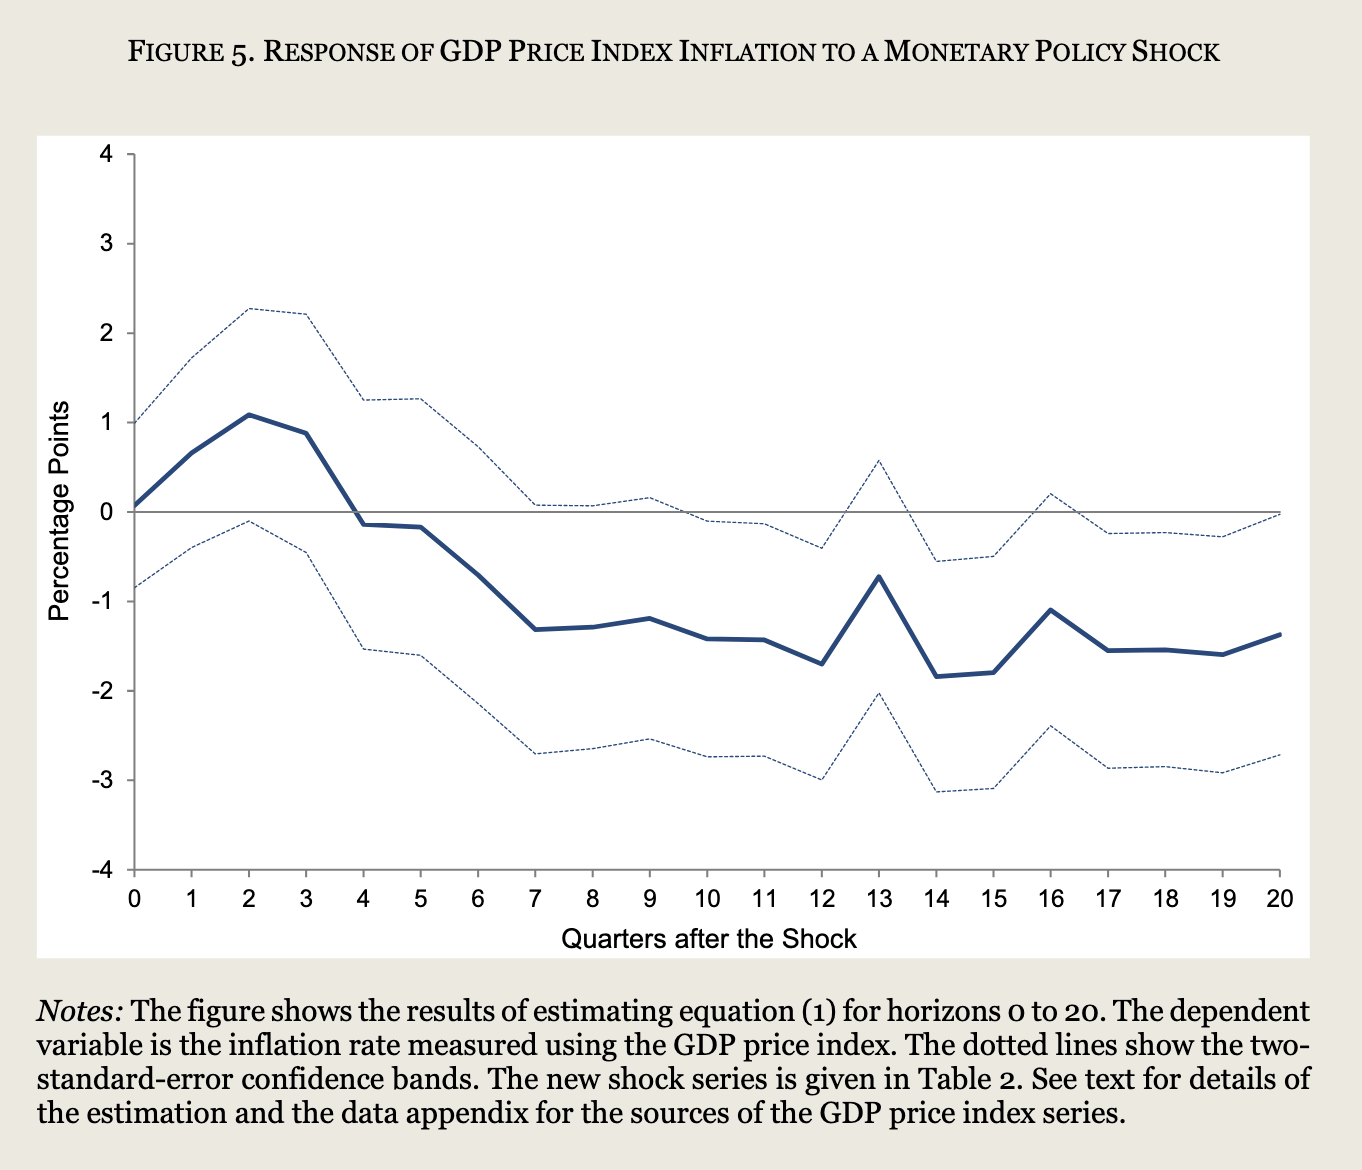
\includegraphics[height=1\textheight]{Graphs/GDPIndexInflation Response.png}
\end{frame}

\begin{frame}{Response of GDP}
  \begin{itemize}
    \item GDP ↓ by 4.4\% after 9 quarters
  \end{itemize}
    \centering
  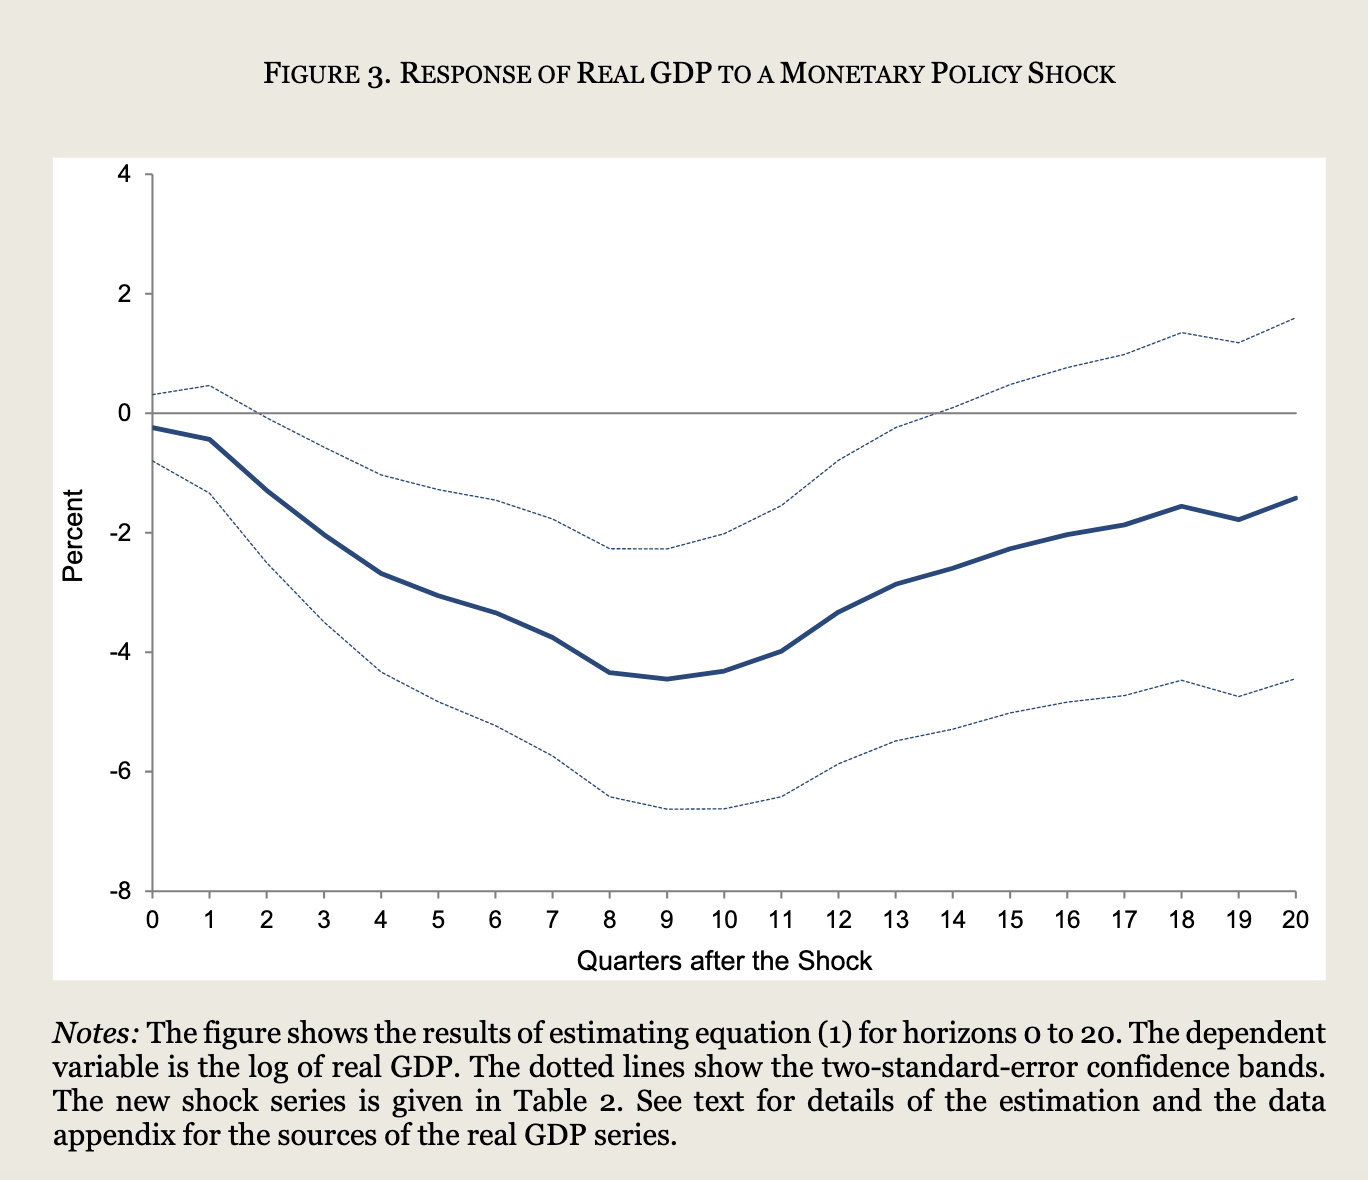
\includegraphics[height=1\textheight]{Graphs/RealGDP Response.png}
\end{frame}

\begin{frame}{Robustness Checks}
  \begin{itemize}
    \item Different inflation indices (PCE, Core PCE)
  \end{itemize}
    \centering
  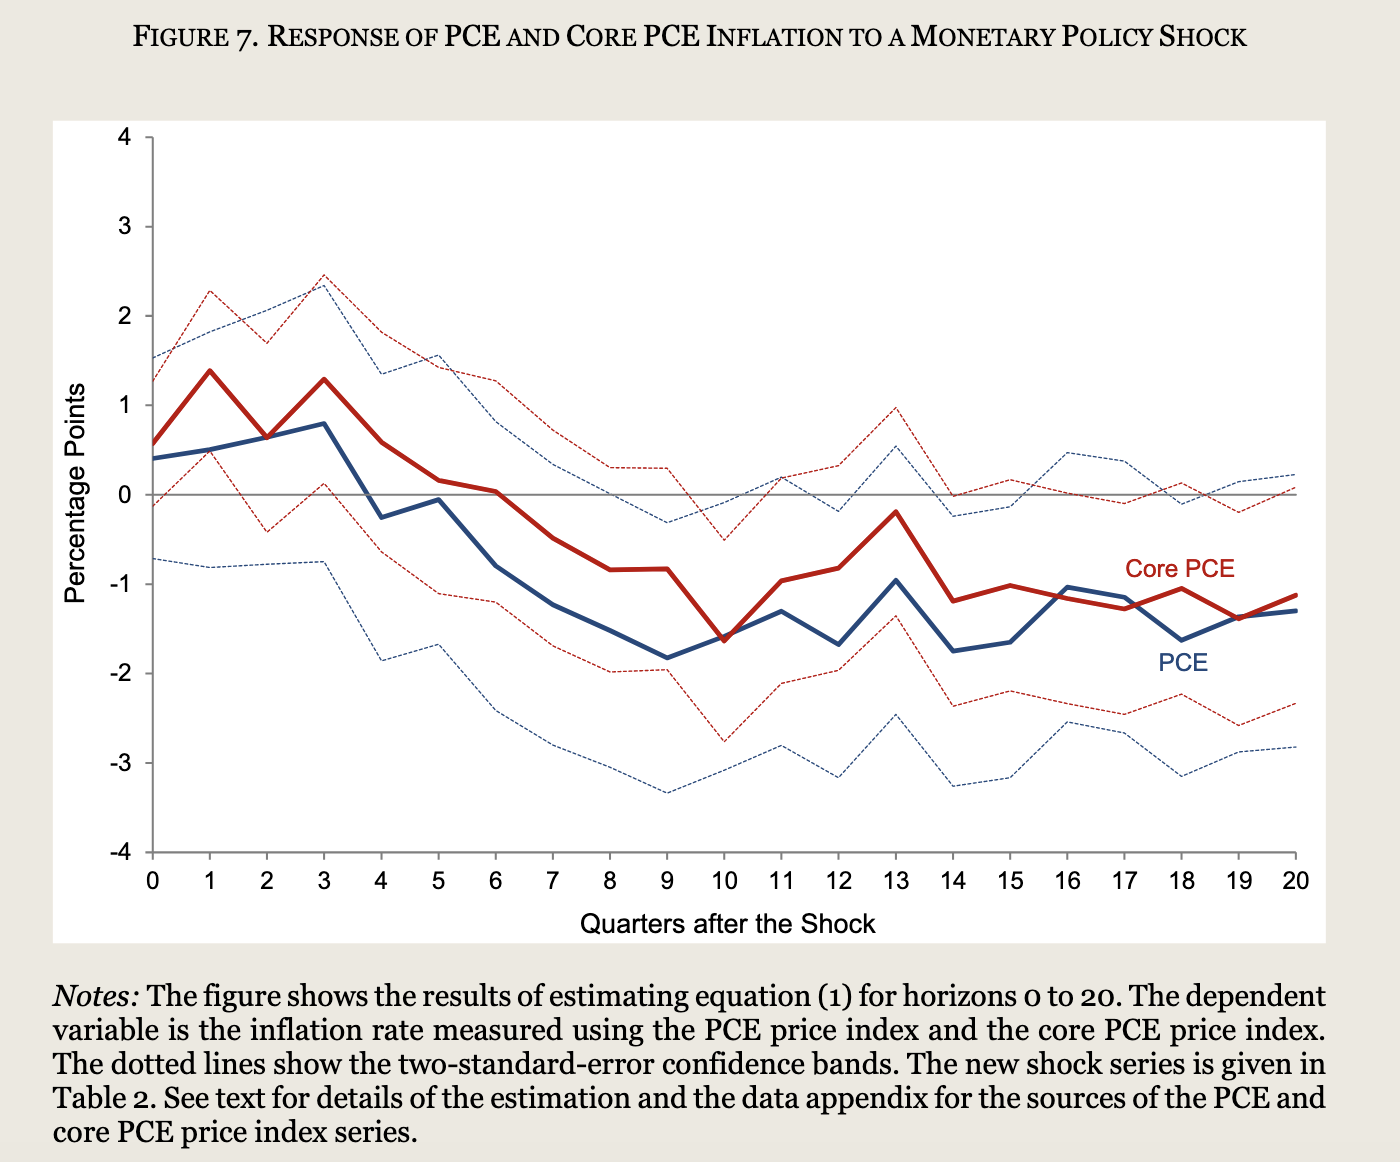
\includegraphics[height=1\textheight]{Graphs/PCE Response.png}
\end{frame}
\begin{frame}{Robustness Checks}
    \begin{itemize}
        \item leave-one-out
    \end{itemize}
    \centering
    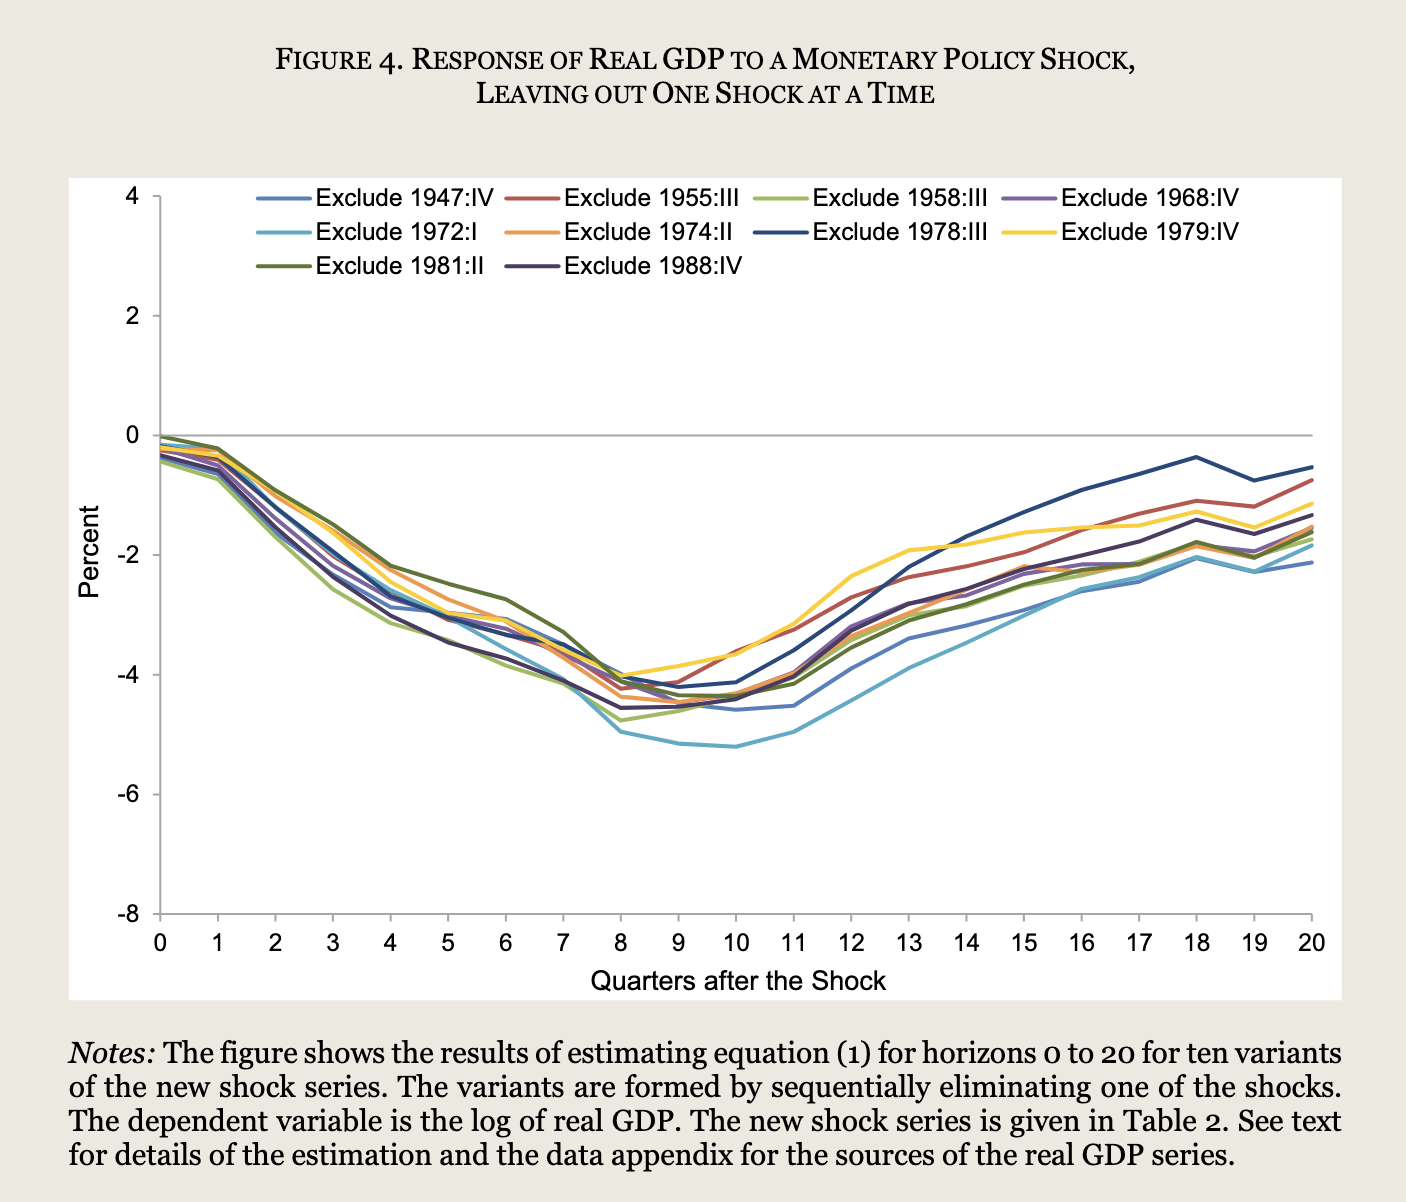
\includegraphics[height=1\textheight]{Graphs/RealGDPRobustness.png}
\end{frame}
% ========== SECTION: Modern Relevance ==========
\section{Modern Relevance}

\begin{frame}{July 2022: Another Exogenous Shock?}
  \begin{itemize}
    \item “Participants observed that inflation remained unacceptably high” (“Minutes,” July 26–27,  2022, p. 8).
    \item Fits Romer-style criteria
    \item However, the inflation rate was already high for months and the real GDP growth rate slowed down.
  \end{itemize}

\end{frame}

\begin{frame}{July 2022: Another Exogenous Shock?}
  \centering
  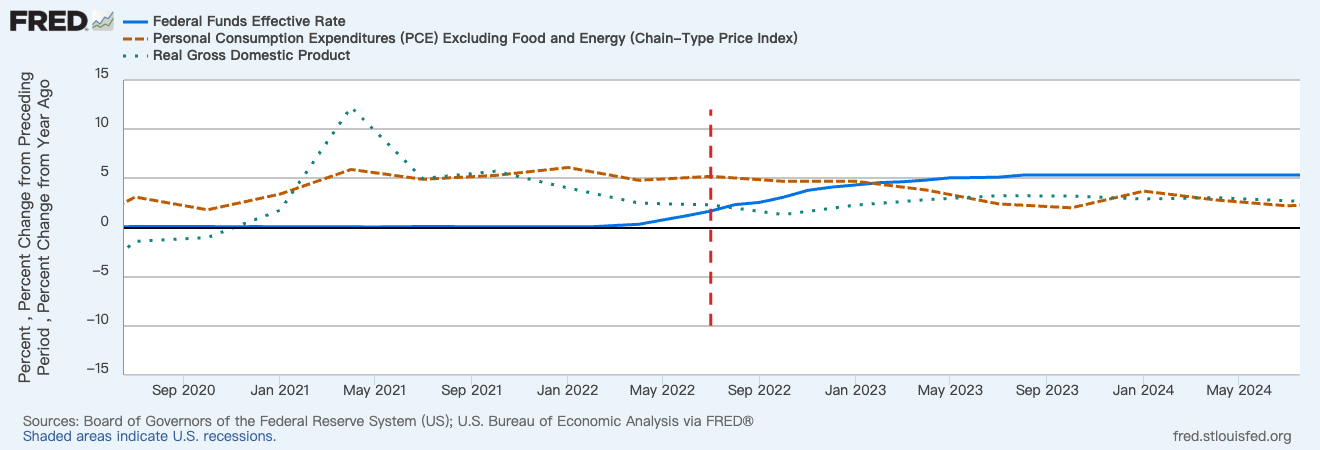
\includegraphics[width=1\linewidth]{Graphs/Jul2022Shocks.png}
\end{frame}
% ========== SECTION: Criticism and Solutions ==========
\section{Criticism and Solutions}

\begin{frame}{Criticism of Narrative Approach}
  \begin{itemize}
    \item Criteria still ambiguous
    \begin{itemize}
        \item Admittedly, it is possible to have a more decisive judgment after reading the full transcripts
    \end{itemize}
    \item Reverse causality risk remains
    \begin{itemize}
        \item The changes in preferences may also be driven by economic conditions, or others things that we do not include in traditional rules, say financial conditions.
    \end{itemize}
    \item No formal counterfactuals
    \begin{itemize}
        \item The narrative approach still does not provide a formal counterfactual for the identified shocks.
    \end{itemize}
  \end{itemize}
\end{frame}
\begin{frame}{Inaction as a Shock?}
  \begin{itemize}
    \item In the 2022 case, the Fed suddenly decided to stop tolerating high inflation and thus was counted as a shock.
    \item Then What about the inaction of the Fed in 2021 when the inflation started to rise?
    \begin{itemize}
        \item But some people argue that the Fed did not change its preference because it believed the inflation was transitory.
        \item Others refered to the so-called ``Make-up''policy, meaning that the Fed was willing to accept higher inflation for a while to make up for the previous low inflation.
    \end{itemize}
    \item Maybe we can also create a new set of criteria for inaction shocks, but it is even harder than identifying action shocks.
  \end{itemize}
\end{frame}
\begin{frame}{Toward Better Identification}
  \begin{itemize}
    \item Use the structural break test to identify exogenous shocks
    \item Explore textual AI 
    \begin{itemize}
        \item However, Romer and Romer mentioned that in some experiments, the correlation between AI-generated results with that by human auditors is very low.
    \end{itemize}
    \item Include the narrative approach in the structural equations estimations
  \end{itemize}
\end{frame}

% ========== SECTION: Conclusion ==========
\section{Conclusion}

\begin{frame}{Key Takeaways}
  \begin{itemize}
    \item Narrative approach solve major identification issues
    \item The empirical results show that Monetary policy has real, lasting effects on the economy
    \item July 2022 may be a modern test case when the full transcripts released in 2027
    \item Narrative approach still evolving and helpful with new models and technologies
  \end{itemize}
\end{frame}
\begin{frame}{Bibliography}
  \begin{itemize}
    \item Romer, Christina D., and David H. Romer. “Does Monetary Policy Matter? The Narrative Approach after 35 Years.” Working Paper. Working Paper Series. National Bureau of Economic Research, April 2023. https://doi.org/10.3386/w31170.
    \item Jordà, Òscar. “Estimation and Inference of Impulse Responses by Local Projections.” American Economic Review 95, no. 1 (March 2005): 161–82. https://doi.org/10.1257/0002828053828518.
  \end{itemize}
  \vspace{1em}
  \textit{Note:} The full transcripts of the FOMC meetings are available at \url{https://www.federalreserve.gov/monetarypolicy/fomc_historical.htm}
\end{frame}
\begin{frame}{Questions?}
  \centering
  \Large Thank you! \\
  \vspace{1em}
\end{frame}

\end{document}